\documentclass[]{elsarticle} %review=doublespace preprint=single 5p=2 column
%%% Begin My package additions %%%%%%%%%%%%%%%%%%%
\usepackage[hyphens]{url}
\usepackage{lineno} % add
\providecommand{\tightlist}{%
  \setlength{\itemsep}{0pt}\setlength{\parskip}{0pt}}

\bibliographystyle{elsarticle-harv}
\biboptions{sort&compress} % For natbib
\usepackage{graphicx}
\usepackage{booktabs} % book-quality tables
%% Redefines the elsarticle footer
%\makeatletter
%\def\ps@pprintTitle{%
% \let\@oddhead\@empty
% \let\@evenhead\@empty
% \def\@oddfoot{\it \hfill\today}%
% \let\@evenfoot\@oddfoot}
%\makeatother

% A modified page layout
\textwidth 6.75in
\oddsidemargin -0.15in
\evensidemargin -0.15in
\textheight 9in
\topmargin -0.5in
%%%%%%%%%%%%%%%% end my additions to header

\usepackage[T1]{fontenc}
\usepackage{lmodern}
\usepackage{amssymb,amsmath}
\usepackage{ifxetex,ifluatex}
\usepackage{fixltx2e} % provides \textsubscript
% use upquote if available, for straight quotes in verbatim environments
\IfFileExists{upquote.sty}{\usepackage{upquote}}{}
\ifnum 0\ifxetex 1\fi\ifluatex 1\fi=0 % if pdftex
  \usepackage[utf8]{inputenc}
\else % if luatex or xelatex
  \usepackage{fontspec}
  \ifxetex
    \usepackage{xltxtra,xunicode}
  \fi
  \defaultfontfeatures{Mapping=tex-text,Scale=MatchLowercase}
  \newcommand{\euro}{€}
\fi
% use microtype if available
\IfFileExists{microtype.sty}{\usepackage{microtype}}{}
\usepackage{graphicx}
% We will generate all images so they have a width \maxwidth. This means
% that they will get their normal width if they fit onto the page, but
% are scaled down if they would overflow the margins.
\makeatletter
\def\maxwidth{\ifdim\Gin@nat@width>\linewidth\linewidth
\else\Gin@nat@width\fi}
\makeatother
\let\Oldincludegraphics\includegraphics
\renewcommand{\includegraphics}[1]{\Oldincludegraphics[width=\maxwidth]{#1}}
\ifxetex
  \usepackage[setpagesize=false, % page size defined by xetex
              unicode=false, % unicode breaks when used with xetex
              xetex]{hyperref}
\else
  \usepackage[unicode=true]{hyperref}
\fi
\hypersetup{breaklinks=true,
            bookmarks=true,
            pdfauthor={},
            pdftitle={It is a good idea to have bad ideas in science.},
            colorlinks=true,
            urlcolor=blue,
            linkcolor=magenta,
            pdfborder={0 0 0}}
\urlstyle{same}  % don't use monospace font for urls
\setlength{\parindent}{0pt}
\setlength{\parskip}{6pt plus 2pt minus 1pt}
\setlength{\emergencystretch}{3em}  % prevent overfull lines
\setcounter{secnumdepth}{0}
% Pandoc toggle for numbering sections (defaults to be off)
\setcounter{secnumdepth}{0}
% Pandoc header


\usepackage[nomarkers]{endfloat}

\begin{document}
\begin{frontmatter}

  \title{It is a good idea to have bad ideas in science.}
    \author[York University and NCEAS, UCSB]{Christopher J. Lortie\corref{c1}}
   \ead{lortie@yorku.ca} 
   \cortext[c1]{Corresponding Author}
      \address[York University]{Biology, 4700 Keele St, Toronto, ON, Canada.}
  
  \begin{abstract}
  There are few truly bad ideas in authentic science. We need to embrace
  science as a process-driven human endeavour to better understand the
  world around us. Products are important, but through better
  transparency, we can leverage ideas, good and bad, ours and others, to
  do better science. In a brief analysis here inspired by a recent
  discussion of the topic and previous introspections by other ecologists,
  it is proposed that whilst it is a good idea to track ideas and all the
  processes that generate outcomes such as publications, there is inherent
  merit in all scientific ideas. That said, organizing and framing our
  ideas into the networks that we already use to examine hypotheses and
  questions in science is a window into our workflows including ideation,
  implementation, data analyses, and how we can better map ideas into open
  science outcomes. Formalizing and describing the linkages between ideas,
  data, and projects we produce as scientists will enhance and diversify
  the value of the work we do individually and collectively.
  \end{abstract}
  
 \end{frontmatter}

\section{Introduction}\label{introduction}

A recent editorial suggests that science is all about sorting the wheat
from the chaff (Kirwan 2017). To be clear and fair, the author
conceptualizes bad ideas using suggestions from eminent scientists on
the value and necessity of bad ideas to the advancement of good science.
It is concluded that successful science must embrace a pluralism of
ideas and that it is not a waste of time to explore ideas that do not
work out. The bad-idea science paradigm proposed is a simple dichotomy
defining good ideas as those that generate publications and bad as those
that do not. This is a functional taxonomy for the purposes of a
self-assessment of work done (i.e.~effort allocated) and project ideas
by the author, and to the defence of this analysis, every effort was
made to qualitatively include ideas that were `built on' for subsequent
positive outcomes, i.e.~publications. This working definition is an
absolutely necessary and convenient short-cut, but it is not the end of
the story. The accountability of ideas to the progress of a discipline
such as ecology is not a new idea (Grime 1993; Weiner 1995) nor without
debate (Aarssen 1997; Weiner 1999). Common ground suggests that we
should individually evaluate the merit of our ideas if for no other
reason then to better prepare our work for the review process of others.
We can even conceptualize some of the less productive ideas as stepping
stones to more useful ones or as a counterpoint to frame and anchor the
relative merit of those that succeed in whatever capacity we elect to
define the positive outcomes. Creation, divine or otherwise, is not a
perfect system. Evolution needs mutations. That ideas are bad if they do
not either directly or indirectly generate publications is perhaps too
limiting. New ideas are novel, and new \emph{and} useful ideas are
creative (Runco and Jaeger 2012). The former can become the subtrate for
the latter. Useless today can become indispensible tomorrow. Sorting the
wheat from the chaff is an exercise in predicting an unknown landscape
of discovery. Introspection of our workflows and the relationship
between ideation and implementation will nonetheless streamline the
mapping of ideas and hypotheses to effective testing through evidence.
However, we also need to ensure that ideas do not get lost through
self-criticism, lack of data, availability of a mechanism to test today,
or through entanglement in the quagmire of extensive information we
process as scientists. In the spirit of replication science (Brandt et
al. 2014; Mulkay and Gilbert 1986), I examined my relative idea
management and outcomes to explore whether this more generous
interpretation of merit and my workflow kept some of the wheat and most
of the chaff.

\section{Methods of replication}\label{methods-of-replication}

A simplified, direct replication of the concept of idea merit
self-assessement from the most recent editorial that inspired this
commentary was done. A check of idea efficacy scrapes the files and
structures used to support a scientific workflow (hosted locally, but
see below on how this landscape is changing). This in and of itself is a
superb idea. The need and pressure to publish can encourage one to be
less cognizant of the processes that support the final paper
particularly if there are many steps or if time to final acceptance is
significant (Powell 2016). Many of the simple rules for data and
experimental provenance (Kazic 2015) also apply to what can be similarly
termed `scientific idea provenance' including version control,
integration, object labelling, and semantics review. The author in the
former idea provenance self-study examined all projects completed in
career, recorded initiation date, scored effort for each, and developed
an outcome classification scale that included direct and indirect
publications from each project (Kirwan 2017). A project was defined as a
`project folder' that likely represented parent directories organized
around each independent research thread. The author concluded that 25\%
of projects generated a publishable result. The assumption of this
workflow is that every scientific task is assigned to/nested within a
project folder. The folder dimension of my scientific workflows is
similar but not a perfect match (and it is fundamentally evolving). I
use project folders to organize protocols and ideas, dataset folders for
data and some other forms of scientific evidence such as camera trap
pictures, an `idea archive' parent folder to store all ideas, and a
`papers-in-progress' parent folder with subfolders to store ideas that
have some development in written form. However, this workflow and
structure for organzing the processes that support scientific inquiry is
dramatically changing thanks to GitHub and RStudio where I couple code,
annotation, and written interpretations with the associated datasets.
Scoring effort and time allocated, pre-Github and without effective,
time-stamped version control was not viable in terms of reproducibility
with my former workflow and its files. Consequently, I restricted
analyses primarily to counts. However, I propose that the number of
objects within a project, i.e.~files, in addition to parent/child
folders that support a research thread is an important building block in
many instances in the process of turning ideas into more tangible
outcomes. This conceptualization of project workflows more fully
embraces a provenance paradigm for ideas. Hence, I use a more
topological approach to model the merit of ideas herein but expanded the
supporting structures associated with ideas and workflows. The diversity
of outcomes can also be expanded to recognize open science products
published online such as datasets in recognized repositories, slide
decks in hosting services, and code that supports data and traditional
publications.

To provide context for the idea provenance self-study, I did a scrape of
scientific outcomes published online. Papers were recorded as positive
outcomes if in print with a peer-reviewed journal, but pre-prints were
excluded to avoid non-independence issues. The count of papers was the
primary outcome used as the denominator in the previous examination
(Kirwan 2017). Datasets published with a DOI in a repository, open slide
decks published online with a recognized sharing service, independent
repositories with code and data posted to GitHub, and other open science
products such as conceptual figures on figshare were also recorded.
Total number of independent ideas stored within a parent directory on my
local HD were also included in this examination as an estimate of the
total available seed pool for all these public outcomes, i.e.~from the
seeds to the established wheat plants. This more inclusive, open science
perspective on outcomes showed that traditional peer-reviewed papers
ranked second after the open science products category (Figure 1). This
is likely representative of many scientists because we give many talks,
and if a slide deck was posted online for many of them, it would exceed
the number of publications. Conceptual figures or scientific cartoons
are also likely common because many scientists turn predictions or ideas
into a theoretical plot to visualize a relationship during the
experimental design phase of a project. Many of these visual predictions
are unsupported but faciliate `sketching out' the ideas for the final
publication. Finally, the total count of all ideas that I allocated time
to record and formally capture as an individual note within the parent
folder I termed my `idea archive' (that is certainly not a Sherlockian
mind palace) nearly tripled the count of papers published. In my
experiences within working groups, this is within the range of ideas
proposed and formally captured in some written capacity. Many more ideas
are wildly sown in these collaboratively endeavours, but the capture and
germination rate drops off significantly within collective and
individual workflows.

At the local level, processes that support these outcomes were scraped
from my working machine. These fundamental attributes that reflect my
pre-GitHub workflow were comprised of projects (thematic subfolders and
files within a parent research projects directory), datasets (thematic
subfolders and files within a parent datasets directory),
papers-in-progress (subfolders, with files, that in theory will become
submissions to journals), and ideas stored within an idea archive parent
directory as described above. I partition the local drive to separate
operating system files from all working files. The total number of
subfolders and files were counted using the command line for the
evidence drive. Subfolders is the closest approximation to the previous
idea provenance examination. For my specific digital workflow, this
level best approximates independent research projects because evidence
or ideas are typically aggregated into outcomes that can become
publications using these topic subfolders. For instance, there were a
total of 79 papers-in-progress subfolders and each includes some writing
that is the germinant of a potential paper. There were a total of 127
subfolders for datasets with each including sets of experimental data
associated with a specific outcome, i.e.~survey data on an invasive
plant plus a follow-up greenhouse trial within the same subfolder
because they were integrated into the same project/research thread and
thus subsequent paper. There were a total of 75 project subfolders in my
scrape suggesting that I have completed (with colleagues) this number of
different research threads. All data, analyses, and this commentary are
provided within a
\href{https://cjlortie.github.io/bad.ideas/}{\textbf{GitHub repository}
on this topic}. This is not a significant deviation from the workflow of
Kirwan, a rheumatologist. An interesting extension is the count of
number of files within each of these threads that illuminated the extent
that one compiles evidence to explore ideas. Locally stored, there were
4571 datasets, 2005 project files, 804 notes and written documents
within papers-in-progress, and 376 annotated ideas (each within a .txt
file within that specific archival category). To examine the sensitivity
of this scale of provenance, both subfolders (replicating the previous
analysis) and number of files were used to estimate the proportionate
mapping of these scientific elements to published papers (i.e.~126 to
date). There was significant variation in the mapping or mobilization of
the different building blocks to published papers (Figure 2). The
file-level analysis of ideas that estimates individual, annotated ideas
in my workflow suggests that 33\% of ideas stored locally become papers.
Nearly 60\% of project subfolders became publications whilst every
folder of datasets mapped onto a paper. This is a coarse matching, and
the ideal provenance tracking would trace idea-to-data-to-paper, but in
reality, the process flows both ways with individual datasets also
leading to idea publications without the the data that first inspired
the thread. Data and ideas can both propagate laterally to other data
and ideas, and individual objects need not directly connect to an
outcome to nonetheless promote positive shared outcomes. Discovery, even
by one individual, is unlikely to be a perfect linear mapping process.
It is reasonable to assume from these findings that few ideas can lead
to many data that in turn produce fewer publications. The converse is
also true that many data can reciprocally catalyze fewer ideas, bad or
good.

\section{Implications}\label{implications}

Without digressing into a theory versus data paradigm clash (Zeller and
Carmines 1980), it is legitimate to examine our own scientific
workflows, transparently, to ensure that there are limited impediments
in connecting different forms of scientific inquiry and to further
ensure that ideas are not lost or unduly discarded. We live in a data
deluge wherein we are uninundated with and perhaps as scientists
routinely compelled to collect data. More intriguingly, it is worthwhile
to not only ask can I collect useful data as a scientist, but to revisit
the wheat-chaff metaphor, am I a good (i.e.~reasonable) idea farmer?
Does my process embrace and retain ideas that can support a meaningful,
and at times, evidence-based decision process in mobilizing and
disseminating research from the insights that I possess as an expert? In
this limited methodological replication, an ecologist and rheumatologist
shared similar levels of career-to-date idea provenance respectively
turning 33 and 25\% of ideas into publications - although we did not
have identical workflows because my projects and ideas were stored
separately. This is an experiment of one, twice. This suggests that
different scientists are not entirely dissimilar in how we organize our
scientific processes and the extent that we ideate; however, it would be
ideal to make this process more reproducible and scaleable. Ideas
without context (stored in `idea archive' on a local desktop) rarely
become more than just that - a noted idea visible to one. There is
certainly a need for a venue for ideas that provides both recognition,
context via tags, and discoverablility by others. Many traditional
journals such as Oikos for ecologists have a Forum section as an outlet
for ideas, but these contributions are generally handled as typical
submissions with peer review, expectations associated with extent of
development, and some structure. This can be an impediment to openly
sharing. Ideas in Ecology and Evolution is another outlet that is more
rapid and relatively less structured in accepting ideas, but the outcome
is still a written paper. Many scientists currently also use social
media, conference presentations, and a few other channels to share
ideas, but aggregation and searchability is limited. An idea respository
similar to those for data is just as important and relevant as a
substrate for the advancement of science, reproducibility, and
synthesis.

Many ecologists likely collect a significant volume of independent data
files. This strongly suggests that many objects, i.e.~files, are needed
as building blocks between an idea and an outcome. Most folders I used
to organize these quantitative observations and experiments ultimately
became a publication, but the individual data files were but stepping
stones in the scientific process. Data can embody ideas - bad and good
ones! We must openly publish more of our data to stimulate these
discoveries for others. Recognized open science products (with a DOI)
such as published datasets, data publications, figures, and code
repositories are thus likely both a critical catalyst for new ideas for
similar cognitively-minded scientists and an invaluable outcome in
addition to traditional papers. An alternative perspective is that one
can work backwards from an idea not forward. The idea is the vision and
the principal object, and the data and the experiments are iterations to
explore its merit. For me, data map onto ideas suggesting a cognitive
workflow associated with/grounded in ideation from observation.
Organizing ideas into project folders is a useful approach and some
elements of a workflow that incorporate aggregation likely increases the
capacity for lateral propogation of data and ideas. We should consider
using digital structures that increase the chances of connecting the
dots. Retain ideas and data but ensure there is a focus on connections
and provenance. Scientific synthesis is clearly not just a formal method
we can use to describe the work of others (Lortie 2014) but a critical
tool we need to practice individually. Hence, workflows that stimulate
and faciliate connecting ideas and data into networks will promote more
creative and more integrated science. A diverse crop of ideas and
outcomes is better than just wheat.

\begin{figure}
\centering
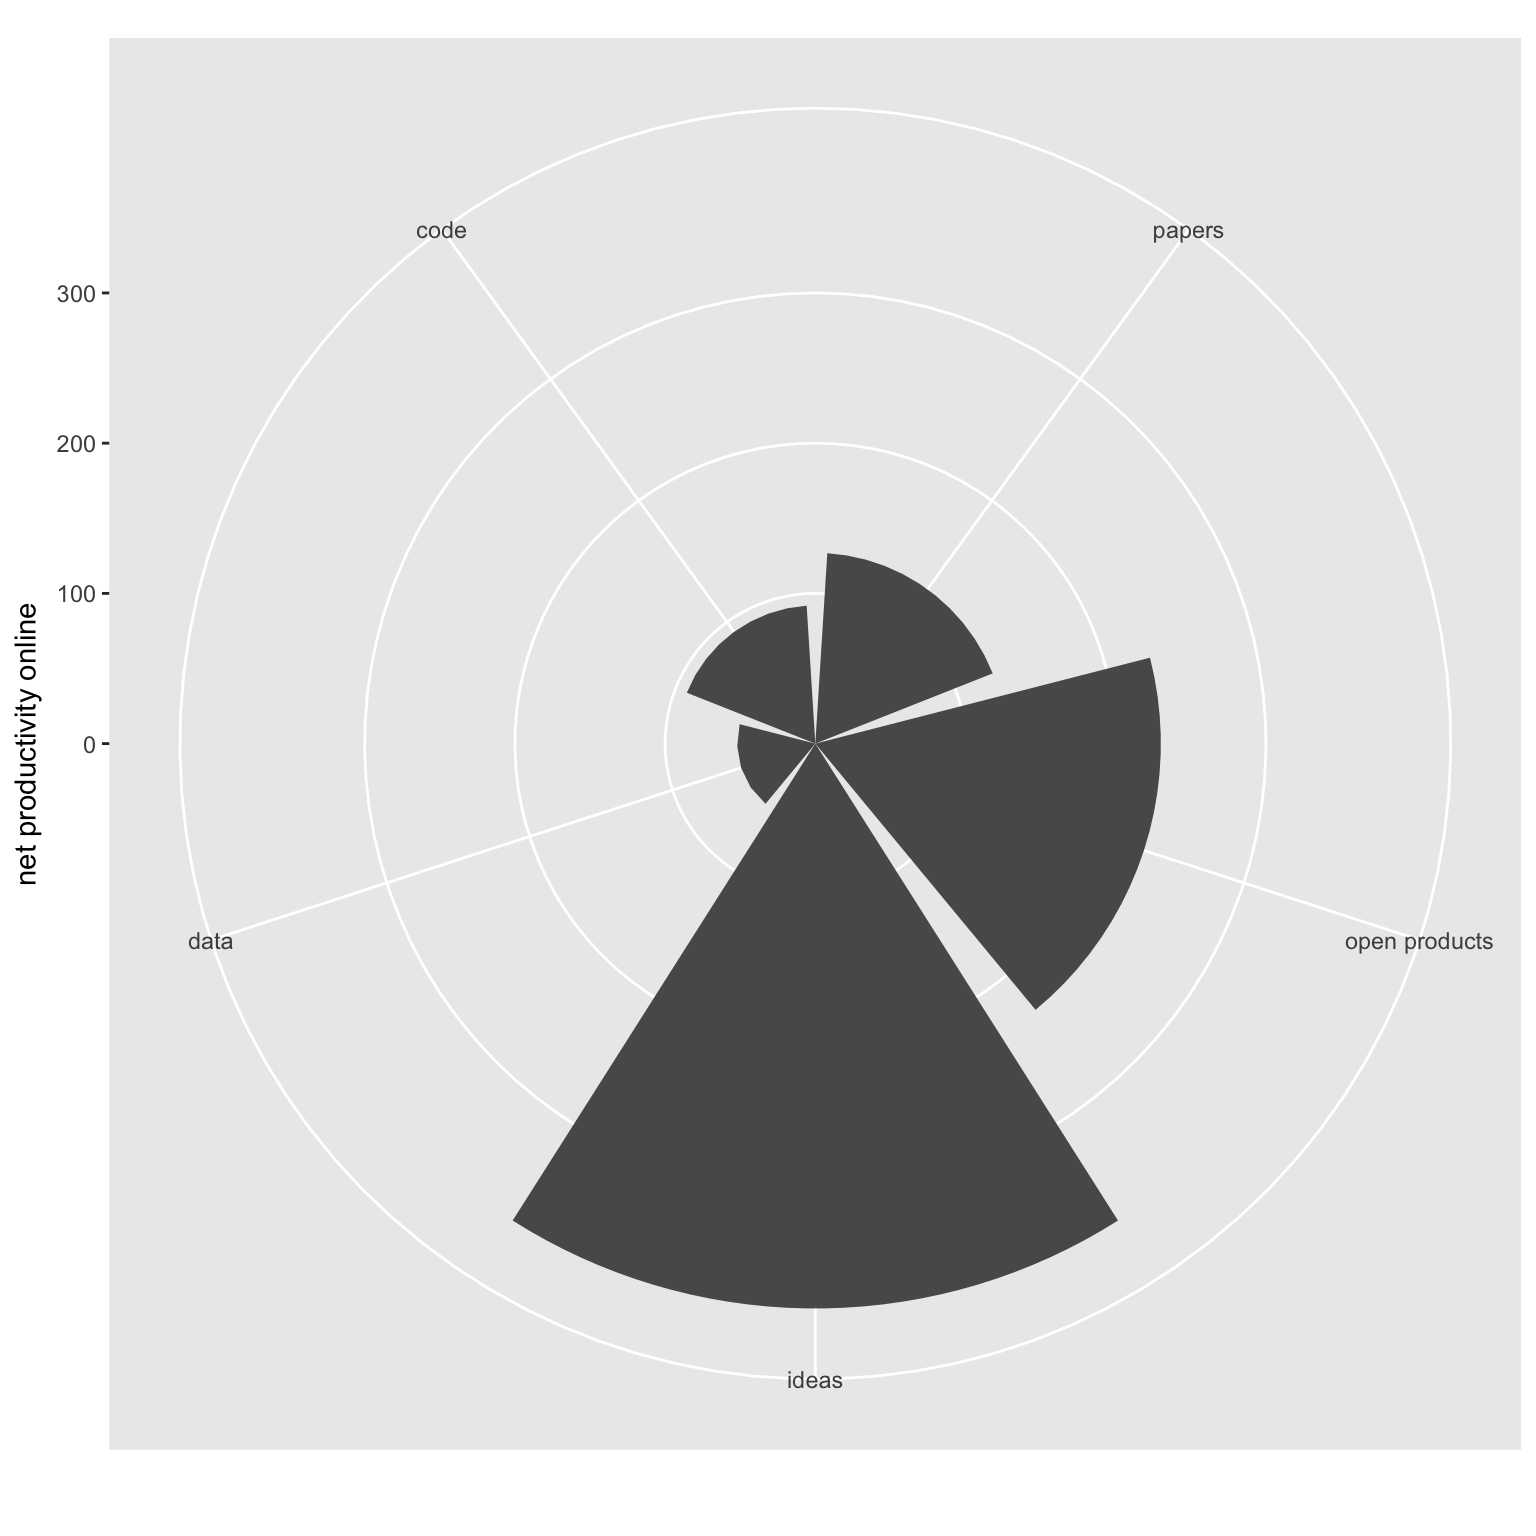
\includegraphics{./fig1.png}
\caption{Scientific outcomes published online and ideas captured locally
within a collective career-level scrape of productivity for an
ecologist. See text for full description of each scientific element
class. The open products category includes slide decks and figures
posted online in open repositories.}
\end{figure}

\begin{figure}
\centering
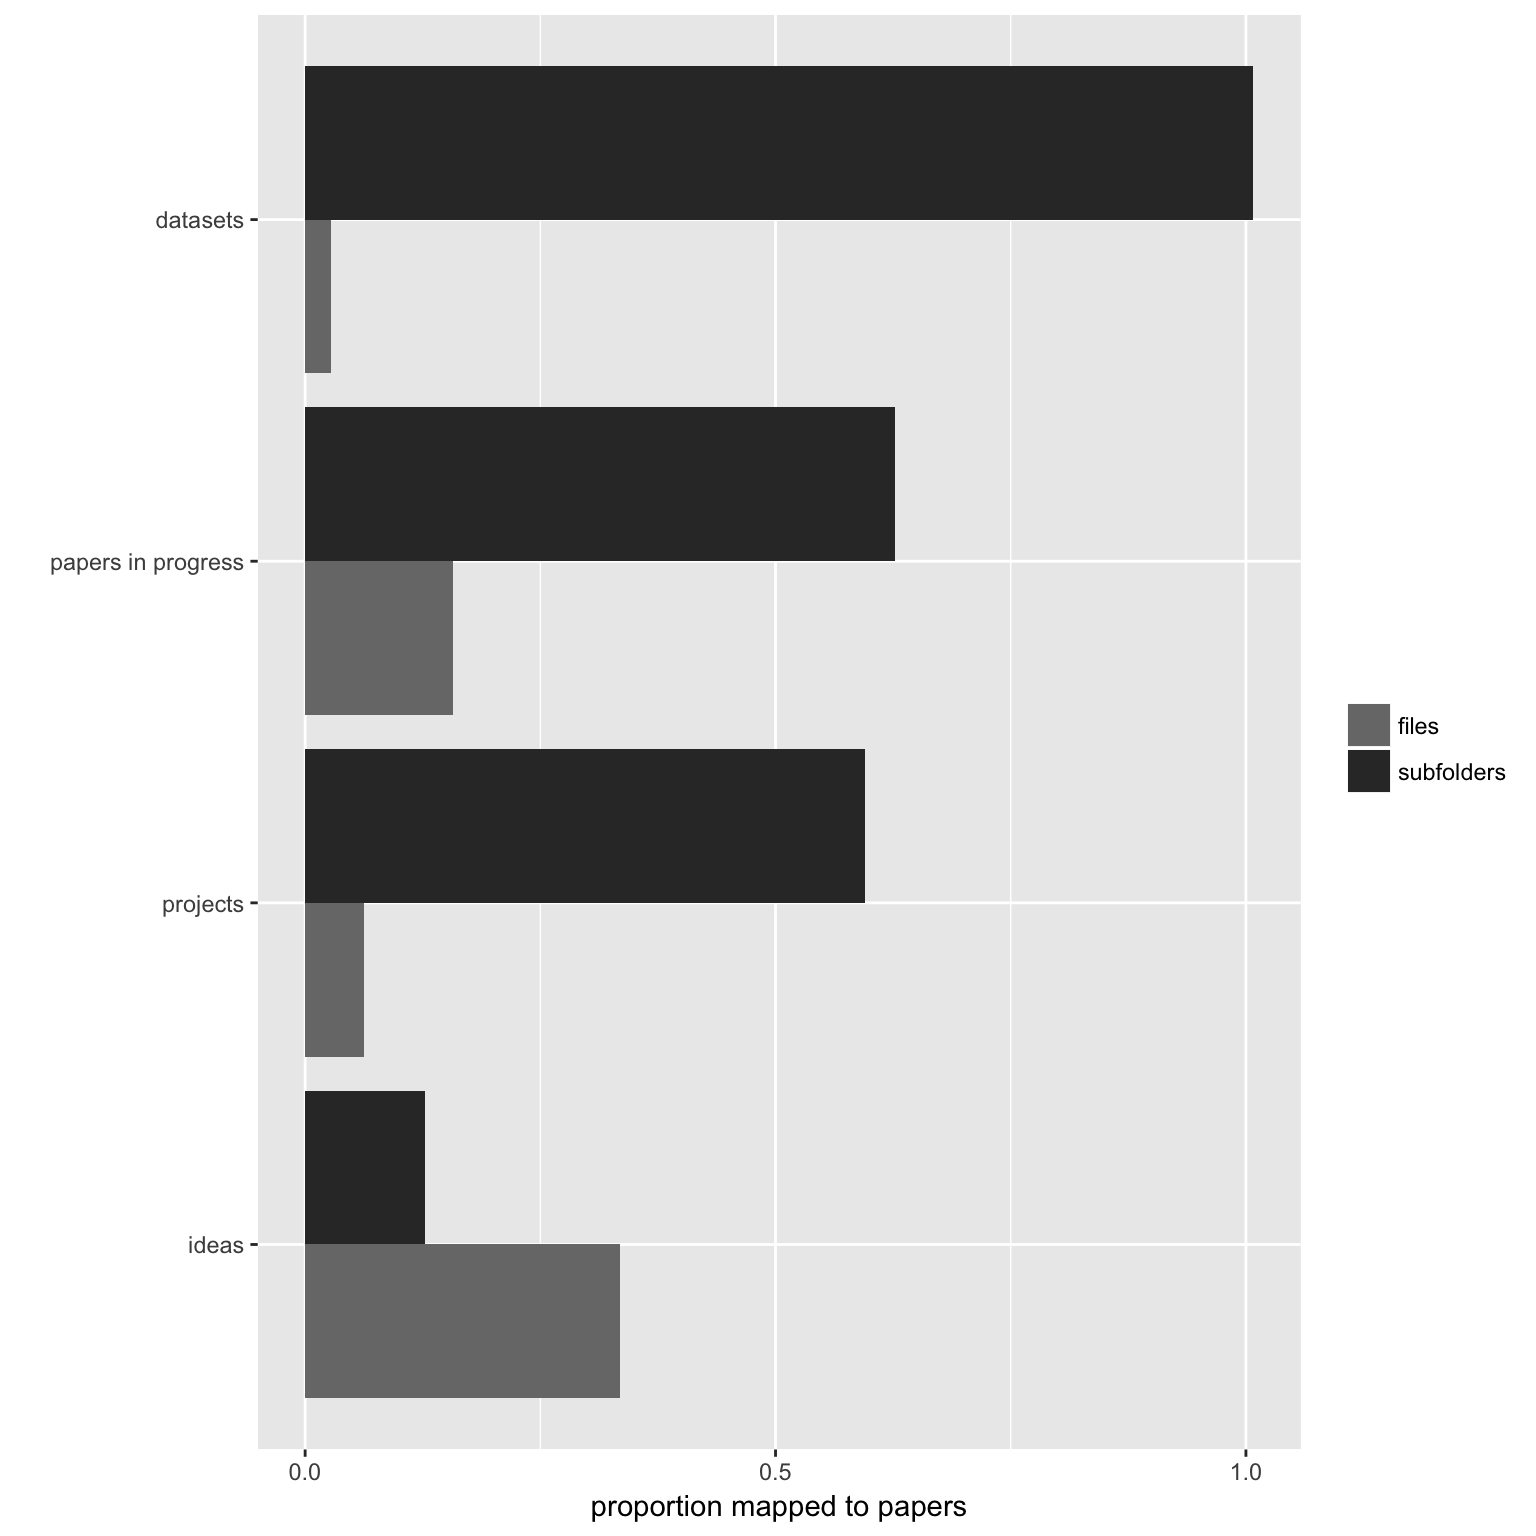
\includegraphics{./fig2.png}
\caption{The mapping of ideas and other supporting research processes
stored locally to peer-reviewed publications in print or press. The
files class represents total number of files stored within a specific
category of research thread, and subfolders were the number of folders
within parent directories stored on working machine for projects, data,
papers-in-progress, and ideas - i.e.~the workflow that an ecologist used
to organize working files for scientific inquiry and experiments.}
\end{figure}

\section*{References}\label{references}
\addcontentsline{toc}{section}{References}

\hypertarget{refs}{}
\hypertarget{ref-Aarssen1997}{}
Aarssen, L.W. 1997. ``On the Progress of Ecology.'' Journal Article.
\emph{Oikos} 80 (1): 177--78.

\hypertarget{ref-Brandt2014}{}
Brandt, Mark J., Hans Ijzerman, Ap Dijksterhuis, Frank J. Farach, Jason
Geller, Roger Giner-Sorolla, James A. Grange, Marco Perugini, Jeffrey R.
Spies, and Anna van 't Veer. 2014. ``The Replication Recipe: What Makes
for a Convincing Replication?'' Journal Article. \emph{Journal of
Experimental Social Psychology} 50: 217--24.
doi:\href{https://doi.org/http://dx.doi.org/10.1016/j.jesp.2013.10.005}{http://dx.doi.org/10.1016/j.jesp.2013.10.005}.

\hypertarget{ref-Grime1993}{}
Grime, J.P. 1993. ``Ecology Sans Frontieres.'' Journal Article.
\emph{Oikos} 68: 385--92.

\hypertarget{ref-Kazic2015}{}
Kazic, Toni. 2015. ``Ten Simple Rules for Experiments' Provenance.''
Journal Article. \emph{PLoS Comput Biol} 11 (10): e1004384.
doi:\href{https://doi.org/10.1371/journal.pcbi.1004384}{10.1371/journal.pcbi.1004384}.

\hypertarget{ref-Kirwan2017}{}
Kirwan, J. 2017. ``It's Good to Have Lots of Bad Ideas.'' Journal
Article. \emph{Nature} 548: 491.
doi:\href{https://doi.org/10.1038/nj7668-491a}{10.1038/nj7668-491a}.

\hypertarget{ref-Lortie2014}{}
Lortie, C. J. 2014. ``Formalized Synthesis Opportunities for Ecology:
Systematic Reviews and Meta-Analyses.'' Journal Article. \emph{Oikos}
123: 897--902.

\hypertarget{ref-Mulkay1986}{}
Mulkay, Michael, and G. Nigel Gilbert. 1986. ``Replication and Mere
Replication.'' Journal Article. \emph{Philosophy of the Social Sciences}
16 (1): 21--37.
doi:\href{https://doi.org/10.1177/004839318601600102}{10.1177/004839318601600102}.

\hypertarget{ref-Powell2016}{}
Powell, K. 2016. ``The Waiting Vame.'' Journal Article. \emph{Nature}
530: 148--51.

\hypertarget{ref-Runco2012}{}
Runco, M.A., and G.J. Jaeger. 2012. ``The Standard Definition of
Creativity.'' Journal Article. \emph{Creativity Research Journal} 24:
92--96.

\hypertarget{ref-Weiner1995}{}
Weiner, J. 1995. ``On the Practice of Ecology.'' Journal Article.
\emph{Journal of Ecology} 83: 153--58.

\hypertarget{ref-Weiner1999}{}
---------. 1999. ``On Self-Criticism in Ecology.'' Journal Article.
\emph{Oikos} 85 (2): 373--74.

\hypertarget{ref-Zeller1980}{}
Zeller, R.A., and E.G. Carmines. 1980. \emph{Measurement in the Social
Sciences. the Link Between Theory and Data.} Book. New York: Cambridge
University Press.

\end{document}


